% Preamble
\documentclass[11pt]{PyRollDocs}
\usepackage{textcomp}

\addbibresource{refs.bib}

% Document
\begin{document}

    \title{The Marini Spreading PyRoll Plugin}
    \author{Christoph Renzing}
    \date{\today}

    \maketitle

    This plugin provides a spreading modelling approach with Marini's formula for flat rolling, adapted on groove rolling by an equivalent rectangle approach.


    \section{Model approach}\label{sec:model-approach}

    \subsection{Marini's spread equation}\label{subsec:marinis's-spread-equation}

    \textcite{Marini1941} proposed \autoref{eq:marini} for estimation of spreading in flat rolling.
    Where $h$ and $b$ are height and width of the workpiece with the indices 0 and 1 denoting the incoming respectively the outgoing profile.
    $A$ and $B$ are parameters introduced by Marini.
    $R$ is the roll radius and $\mu$ is the friction coefficient.


    \begin{equation}
        A = \frac{\sqrt{\Delta h}}{2 * \mu * \sqrt{R}}
        \label{eq:marini-parameter-a}
    \end{equation}

    \begin{equation}
        B = \sqrt{\frac{\Delta h}{R}}
        \label{eq:marini-parameter-b}
    \end{equation}

    \begin{equation}
        b_1 = b_0 + \frac{2 * \Delta h b_0 \left( R - \frac{h_0}{2} \right) B }{h_1 b_0 + \left( \frac{b_0 \left( h_0 + h_1 \right)}{2} \frac{1 + A}{1 - A} \right) \frac{0.91 \left( b_0 + 3 h_0 \right)}{4 h_0} + 2 h_1 R B}
        \label{eq:marini}
    \end{equation}

    \subsection{Equivalent rectangle approach}\label{subsec:equivalent-rectangle-approach}

    Marini's spreading model~\cite{Marini1941} was originally built for flat rolling.
    A common approach for groove rolling is to calculate some equivalent rectangular profile to be able to use flat rolling models~\cite{Hensel1978, Spittel1984}.
    \autoref{fig:equivalent_rectangle} shows 3 variants of calculating an equivalent rectangle of a profile.

    \begin{figure}
        \centering
        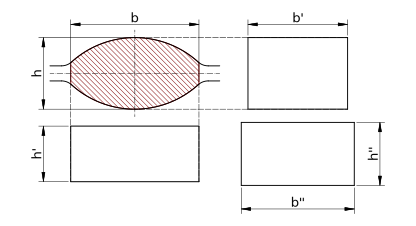
\includegraphics[width=\linewidth]{equivalent_rectangle}
        \caption{Three methods of defining an equivalent rectangle of an oval groove}
        \label{fig:equivalent_rectangle}
    \end{figure}

    The first variant is to keep the width constant and calculate the height $h'$ so that the cross section $A$ is
    equal:

    \[
        h' = \frac{A}{b}
    \]

    The second variant is to keep the height constant and calculate the width $b'$ so that the cross section $A$ is
    equal:

    \[
        b' = \frac{A}{h}
    \]

    Both represent the geometry of the profile poorly.
    A better way is to keep the aspect ratio equal as propose by \textcite{Spittel1984}:

    \[
        h'' = \sqrt{\frac{A h}{b}}
    \]

    \[
        b'' = \sqrt{\frac{A b}{h}}
    \]

    This variant is used in the current implementation.
    So $h$ and $b$ in Wusatowski's model are replaced with $h''$ and $b''$.
    In the end, $b_1$ can be obtained from $b_1''$ by:

    \[
        b_1 = \frac{b_1'' h_1}{h_1''}
    \]


    \section{Usage instructions}\label{sec:usage-instructions}

    The plugin can be loaded under the name \texttt{pyroll\_marini\_spreading}.

    An implementation of the \lstinline{width_change} hook on \lstinline{RollPass} is provided,
    calculating the spread using the equivalent rectangle approach and Marini's model.

    Several additional hooks on \lstinline{RollPass} are defined, which are used in spread calculation, as listed in \autoref{tab:hookspecs}.
    Base implementations of them are provided, so it should work out of the box.
    For \lstinline{marini_parameter_a} and \lstinline{marini_parameter_b} the equations~\ref{eq:marini-parameter-a} and~\ref{eq:marini-parameter-b} are implemented.
    Friction coefficient can be adjusted individually.
    Provide your own hook implementations or set attributes on the \lstinline{RollPass} instances to alter the spreading behavior.

    \begin{table}
        \centering
        \caption{Hooks specified by this plugin. Symbols as in \autoref{eq:marini}.}
        \label{tab:hookspecs}
        \begin{tabular}{ll}
            \toprule
            Hook name                     & Meaning                                      \\
            \midrule
            \texttt{marini\_parameter\_a}   & Parameter $A$ of Marini's spreading equation \\
            \texttt{marini\_parameter\_b}   & Parameter $B$ of Marini's spreading equation \\
            \texttt{friction\_coefficient} & Friction coefficient $\mu$                   \\
            \bottomrule
        \end{tabular}
    \end{table}

    \printbibliography

\end{document}